\section{Conclusion}


\begin{frame} {}

Cet article a donc présenté une solution au problème de conception
de trajectoire d'un drone équipés de système de communication sans fil
en vu de transmettre un fichier à un ensemble de récepteurs i.e. Terminaux Terrestres. 
La mission doit être accomplie en un temps minimum tout en assurant une bonne réception
du message avec une probabilité minimale.

\end{frame}

\begin{frame} {}
 Pour ce faire, plusieurs étapes ont été nécessaires\pause

\begin{enumerate}
	\item Reformulation du problème en utilisant une seule contrainte
	de temps minimum de connexion entre le drone et le terminal terrestre.\pause
	
	\item Les auteurs ont ensuite montré que la trajectoire optimale
	peut-être constituée uniquement de segments de droites reliant des
	waypoints dont la position est optimisée.\pause
	\item Ils ont calculé la position optimale de ces waypoints.
	Ce qui définit une trajectoire optimale. \pause  
	\item Puis ils optimisent la vitesse en fonction du temps le long de la trajectoire obtenue
	en utilisant la programmation linéaire(LP).\pause
	\item Les résultats numériques ont mis en évidence des performances significativement améliorées
	 par rapport à une approche heuristique de conception de trajectoires ou un système multicast statique.\pause
	\item Ce qui tend à montrer le grand potentiel des drones de 
	télécommunication à usage de transmetteurs multicast dans les réseaux sans-fil.
	 
\end{enumerate}
\end{frame}


\begin{frame} {Perspectives}

Dans les systèmes multicast, on peut utiliser un processus de partage de fichiers,
dit device to device (D2D), durant lequel les terminaux terrestres
s'échangent des paquets reçu pendant la phase multicast pour reconstituer leurs messages
respectifs dans leur totalité. 

 \begin{figure}[t]
	\centering
	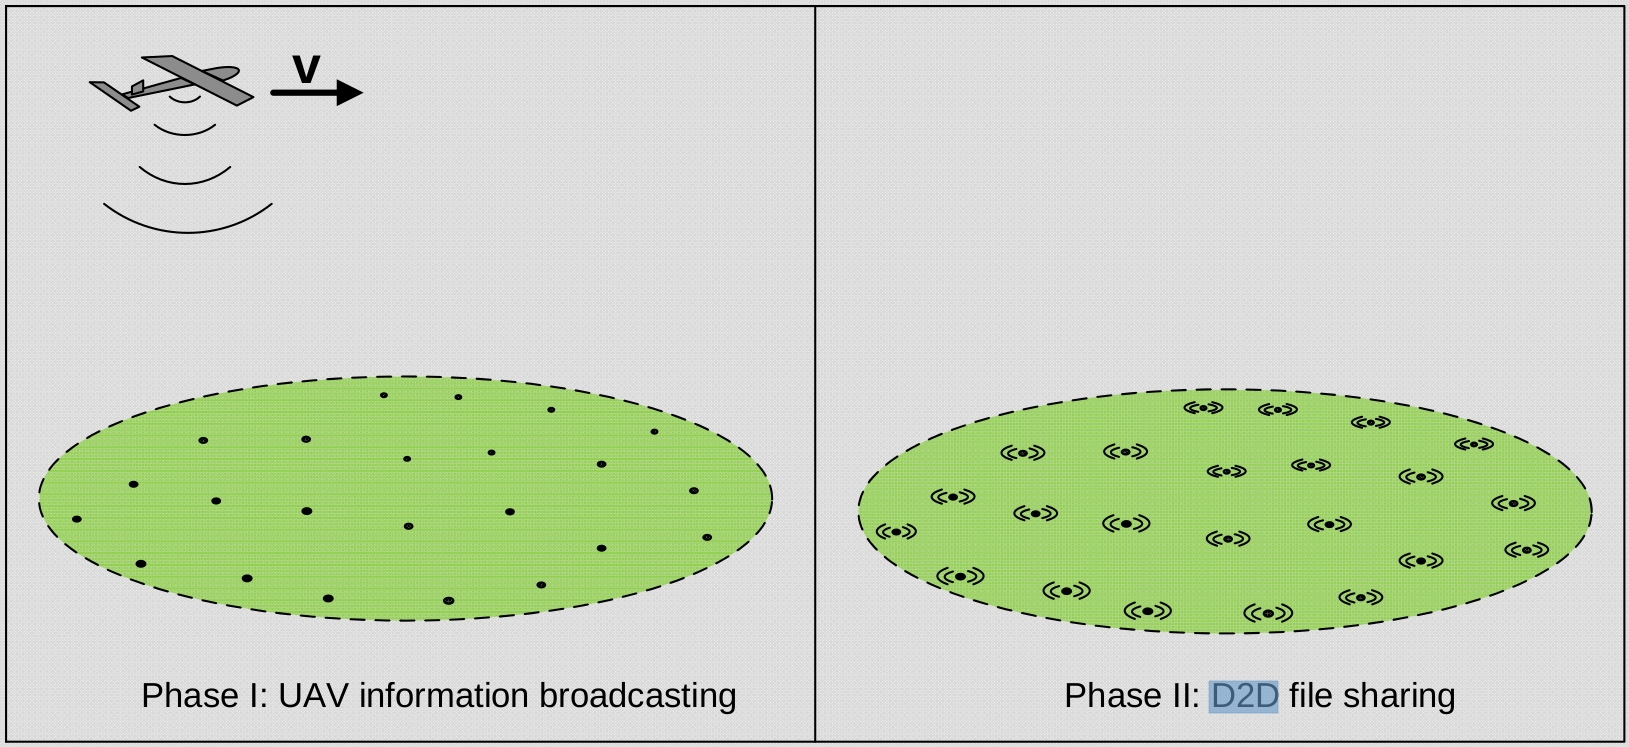
\includegraphics[height=\dimexpr11\textheight/16\relax]{d2d}
	\caption{D2D}
\end{figure}

\end{frame}


\begin{frame} {}

Cet article n'a pris en compte que la phase multicast. L'étude conjointe
des deux phases multicast et D2D serait probablement intéressante à entreprendre.
En lien avec des techniques de clustering pour les stations sol, l'optimisation
conjointe pourrait permettre de réduire davantage les coûts de transmission et donc la taille des drones
utilisés.

\end{frame}